\chapter{Implementation\label{cha:chapter4}}

This chapter describes the implementation of the RDF instances generator and visualizer. 
Three systems were chosen as reference implementations: a VSCode version, a IntelliJ IDEA version and a Browser version. 
\section{Environment\label{sec:env}}
The following software, respectively operating systems, were used for the implementation:

\subsection{Software and development tools\label{sec:os}}

\begin{itemize}
  \item MacOS Sequoia: used during the entire development process as main Operative System.
  \item Windows 11: used to test the extension for VSCode and IntelliJ installed in a Windows environment.
  \item Visual Studio Code: used to develop the web service and the VSCode extension.
  \item IntelliJ IDEA: used for the development of the IntelliJ IDEA extension.
  \item Docker: used to create a virtual environment for the web service.
  \end{itemize}

\subsection{Programming languages, SDKs, and libraries\label{sec:proglang}}

\begin{itemize}
    \item Yeoman and VSCode Extension Generator: used to scaffold a TypeScript project ready for development.
		\item TypeScript and Node.js: used as primary programming language and package management for the VSCode extension.
		\item Kotlin and Gradle: used for the development and packaging of the IntelliJ IDEA extension.
		\item Python and pip: used for the implementation and package management of the web service.
		\item FastAPI: main Python library for the creation of a REST web service.
		\item rdflib: Python library for handling and processing RDF.
		\item sparqlwrapper: library that simplifies the use of SPARQL in Python. 
		\item vis.js: JavaScript library for creating interactive RDF graphs.
\end{itemize}

\section{Project Structure\label{sec:projectstructure}}

The implementation is separated into 3 distinguished projects as depicted in figure \ref{fig:projectstructure}.

\begin{figure}[htb]
  \centering
  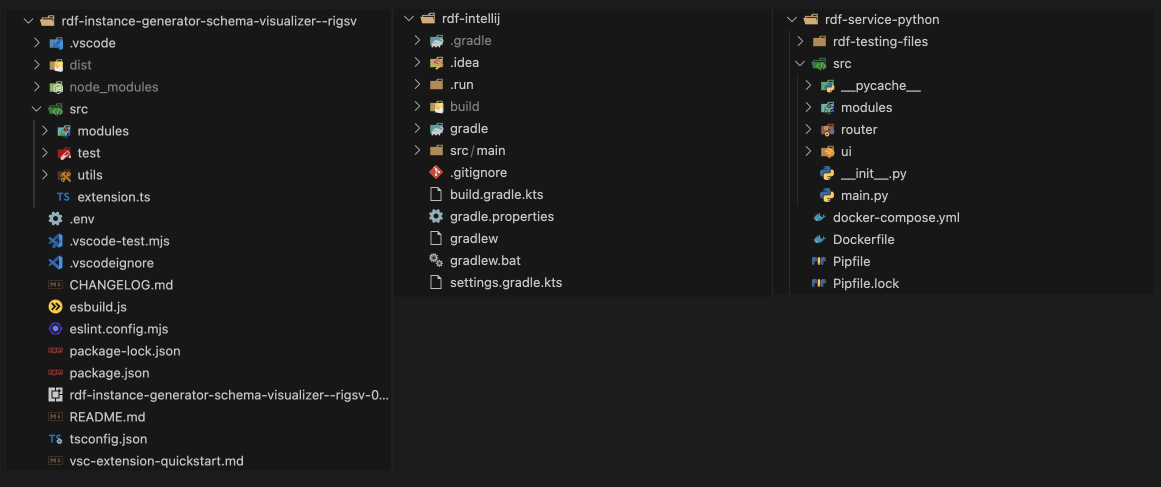
\includegraphics[width=13cm]{folder_structure.png}
  \caption{Project Structure}
  \label{fig:projectstructure}
\end{figure}

The first project is the web service (rdf-service-python), the second one is the VSCode extension (rdf-instance-generator-schema-visualizer--rigvs) and the last one is the IntelliJ plugin (rdf-IntelliJ).

\section{Implementation of the Web Service\label{sec:webservice}}

\begin{figure}[htb]
	\centering
	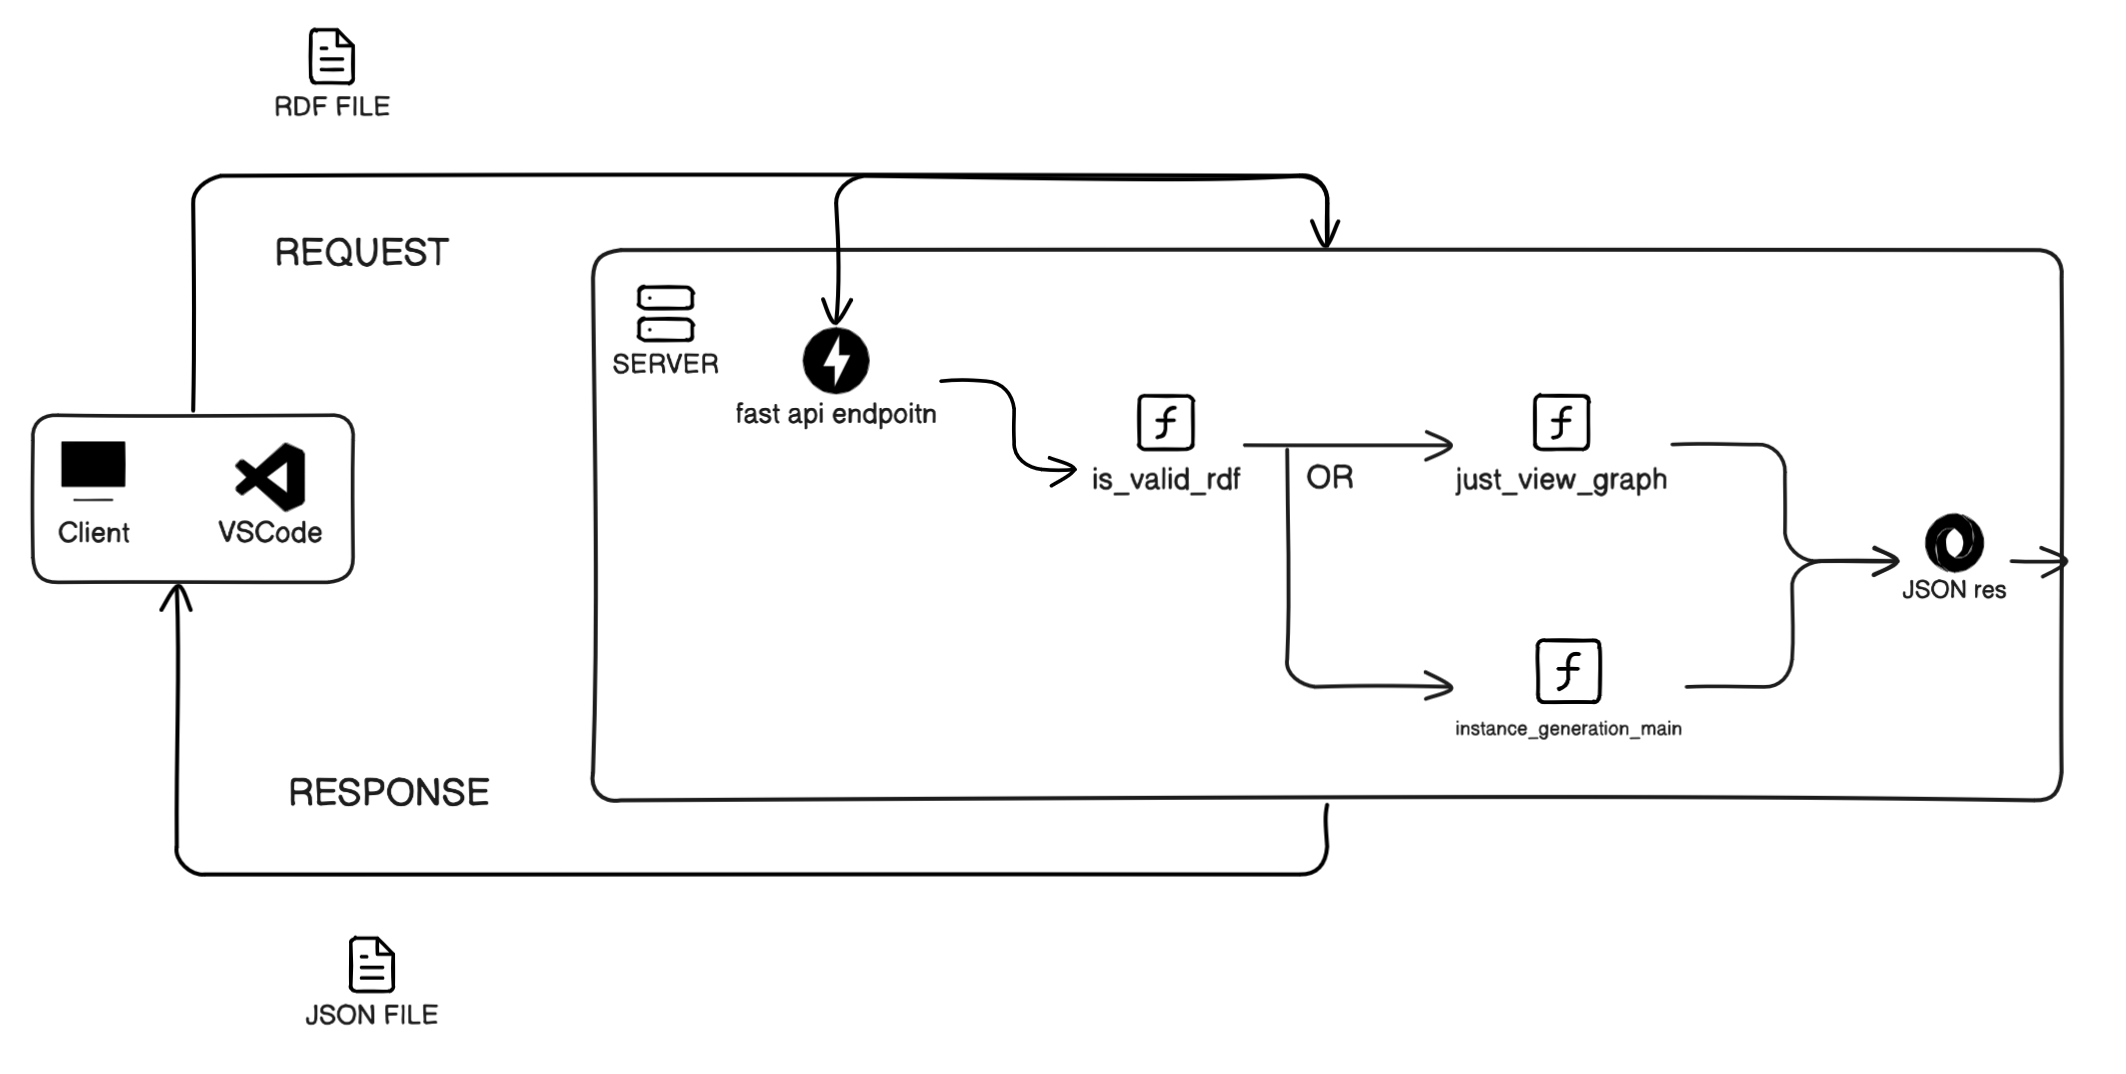
\includegraphics[width=13cm]{server_schema.png}
	\caption{Server Schema}
	\label{fig:serverschema}
  \end{figure}


\noindent
The following section describes in details the implementation of the web service with all its key components.
\\
\\
\subsection{Server} 
There are many Python libraries that allow to create a REST web service. Among them, FastAPI was the chosen one. It is a modern, fast (high-performance), web framework for building APIs with Python based on standard Python type hints \cite{fastapi}.
\\
The first step, in order to start the server, was to install FastAPI and its dependencies. After than, by simplying initializing the app object, \textbf{app = FastAPI()} and execute the \textbf{fastapi dev src/main.py} command, the server will be up and running. 
\\
\\
The next step was to create the endpoints. In src/router/router.py, the \textbf{router = APIRouter()} was initialized and three endpoints where created: to for the Browser Client and one for the extensions.
\\
\\
The first endpoint, \textbf{$router.get("/", response\_class=HTMLResponse)$}, is simply used to server the index.html file to the web Browser. This page allows the upload of RDF (POST to the next endpoint), visualize the generated graph and see the RDF file with the new generated instances.
\\
\\
The next endpoint is the \textbf{$router.post("/generate", tags=["users"])$}. This endpoint accepts incoming POST requests from the Web Browser with the incoming RDF file. It returns the required data in a JSON format.
\\
\\
The last endpoint, \textbf{$router.post("/", response\_class=JSONResponse)$}, accepts incoming POST requests from the VSCode and IntelliJ extensions. It returns data in a JSON format.
\\
\\
\subsection{RDF Validation} 
When an endpoint function receive an RDF file, the first function to be called is the \textbf{$is\_valid\_rdf(file)$}. This asynchronous function is responsible for validating the incoming RDF file. First it extracts the file extension from the incoming file. The extension name must be present in the predefined dictionary. If it's not there, an error is returned otherwise it proceed to the next step.
\\
To see if the code in the file is correct syntactically and semantically, the function uses the \textbf{rdflib} library. This function allows to parsing and serialization of RDF data, storing of RDF triples, accessing to remote SPARQL endpoints, and working with RDF graphs \cite{rdflib}.
The core of this function relies heavily on the $Graph.parse()$ method. If the file is syntactically correct and a new RDF graph is generated, then it means that the RDF is valid and the function returns true. Otherwise, it returns false.
\subsection{Graph generator}
After verifying the file is valid, the next step was to create the actual graph generation function. The $getGraph()$ uses the previously stated method for parsing the RDF file and return the graph, the file extension name and file format name to the $just\_view\_graph()$ function. 
\\
The retrieved graph is then serialized in the requested format and in json-ld.

\subsection{Instance and Graph generator}
This was the most important and complex functionality of the entire project. 
Like it has been done in the previous function, the graph, the format and the extension name are returned from the $getGraph()$.
Then a new graph is initialized and, to keep things consistent and readable, all the namespace prefixes are copied from the initial retrieved graph ($or\_graph$).
This helps make the RDF output cleaner and easier to read, since it avoids repeating long URIs and keeps the format consistent.
\\
\\
The next step is the scanning of the RDF graph. The $scan()$ function goes through the entire graph and extract classes and properties. 
At the start, the $detect_classes()$ function extracts the classes from the graph. Then, the $detect\_properties()$ extracts all the properties and associate their domains and ranges with classes. In conclusion, it ensures that all the classes indirectly referenced are included in the graph.
\\
\\
The code then splits and creates two different functionalities: instance generation without properties search and instance generation with properties search.
\\
\\
In RDF vocabularies, classes can be either explicitly declared (e.g. $rdf:type rdfs:Class$) or implicitly referred with their usages in properties definitions (e.g. $rdfs:range schema:Car$).
In the scenario where the instance generation is executed without the properties search, the code needs to generate and instance for every single class that has been found in the code, both explicitly or implicitly referred. 
\\
The $generate\_instance()$ function, take as parameters the class uri that has been extracted previously, the new graph initialized before, the number of instances that the user wants to generate for each declared class and the properties that has been defined. 
It's important to sate that the user has no control over the number of instances that come from a implicitly referred class.
\\
\\
Once the parameters are set, the function starts by checking i the class uri starts with \textbf{http://www.w3.org/2001/XMLSchema} and in case of a positive answer it skips the instance generation for that class.
\\
\\
After that, the $processed\_instances$ and $initialized\_instances$ are declared. The first, since $generate\_instance$ is a recursive function, is used for tracking which instances have already been generated to avoid duplicates. 
The second tracks which properties have been assigned to each generated instance.
\\
\\
In the next step, the function iterates N times to create multiples instances for the provided class. For each iteration, a new URI is created by using the EX prefix, the class name, and the number of the iteration (e.g. $ex:Employee\_Instance1$). If the instance has already been processed, it is simply reused from $processed\_instances$. The newly created instance is then linked to its class uri and added to the graph. 
\\
\\
If the class has any associated property, the function checks every property and handles three main cases: 
\begin{itemize}
	\item If the provided value is a URI and it is a primitive datatype, thanks to the support of a hashmap (i.e. XSD) containing the primitive types with example values, a new literal is generated and appended to the graph. If the URI is not primitive, it is treated as a reference to another class. The function calls itself recursively to generate the required number of sub-instances for the referenced class. The resulting sub-instance is then added the graph. 
	\item If the value is a XSD datatype URI as string, a default string literal (i.e., "default"^^xsd:string) is generated and the triple added to the graph.
	\item If the value is already a literal it is directly added to the graph.
	\item If the value is unsupported, an error is thrown.
\end{itemize}
Each successful initialized property, is then stored inside $initialized\_instances$.
At the end of the loop, the function adds the generated instance to the instances list and concludes with its return.
\begin{lstlisting}[caption={Instance Generation Function}, label={lst:generate_instance}, language=JavaScript]
	EX = Namespace("http://example.org/")
	
	def generate_instance(
		class_uri,
		graph,
		num_instances=1,
		property_definitions=None,
		processed_instances=None,
		initialized_instances=None,
	):
		from rdflib.namespace import XSD
	
		xsd = {
			"http://www.w3.org/2001/XMLSchema#integer": 0,
			"http://www.w3.org/2001/XMLSchema#decimal": 0.0,
			"http://www.w3.org/2001/XMLSchema#float": 0.0,
			"http://www.w3.org/2001/XMLSchema#double": 0.0,
			"http://www.w3.org/2001/XMLSchema#string": "unknown",
			...
		}
	
		# Skip primitive XSD types
		if str(class_uri).startswith("http://www.w3.org/2001/XMLSchema#"):
			return []
	
		instances = []
		processed_instances = processed_instances or {}
		initialized_instances = initialized_instances or {}
	
		class_name = class_uri.split("/")[-1]
	
		for i in range(num_instances):
			instance_uri = EX[f"{class_name}_Instance{i + 1}"]
	
			if instance_uri in processed_instances:
				instances.append(instance_uri)
				continue
	
			processed_instances[instance_uri] = True
			graph.add((instance_uri, RDF.type, class_uri))
	
			if property_definitions and class_uri in property_definitions:
				for prop, value in property_definitions[class_uri].items():
					if isinstance(value, URIRef):
						if str(value).startswith("http://www.w3.org/2001/XMLSchema#"):
							graph.add((instance_uri, prop,
									   Literal(xsd[str(value)], datatype=value)))
						else:
							sub_instances = generate_instance(
								value,
								graph,
								num_instances=i + 1,
								property_definitions=property_definitions,
								processed_instances=processed_instances,
								initialized_instances=initialized_instances
							)
							if sub_instances:
								value = sub_instances[i]
								graph.add((instance_uri, prop, value))
					elif str(value) in xsd:
						graph.add((instance_uri, prop,
								   Literal(xsd[str(value)], datatype=URIRef(value))))
					elif isinstance(value, Literal):
						graph.add((instance_uri, prop, value))
					else:
						raise ValueError(
							f"Unsupported value type: {type(value)} for property {prop}"
						)
	
					if instance_uri not in initialized_instances:
						initialized_instances[instance_uri] = set()
					initialized_instances[instance_uri].add(prop)
	
			instances.append(instance_uri)
	
		return instances
\end{lstlisting}

In the scenario where the instance generation is executed with the properties search, some previous steps are required before starting the instance generation. 
After the classes' detection, the $find\_properties()$ function is executed. It starts with retrieving all the implicitly referred classes from the list. The function then iterates over the list of URIs and checks if the URI is present in the $vocab$ map (it contains a map of the most common RDF vocabularies). 
Each match is then the passed to the $query()$ function. 
\\
\\
The $query()$ function is responsible for executing the SPARQL query on the LOV (Linked Open Vocabularies) Endpoint and returning the results. It takes three parameters: the class term for which we want to find some properties, the number of properties to retrieve, and the ontology to search in. 
\\
The first step of this function is to build up the SPARQL query for the required ontology (i.e. $fetchQuery()$). Then the query can be executed thanks to the sparqlwrapper library. The results are then polished, filtered and bound to the search class term. At the end, the function randomize the selection of the retrieved property.
\\
In summary, this function helps make automatically generated RDF instances more meaningful by selecting properties that best fit the context of each instance—even when the class hasn’t been explicitly defined in the RDF schema.
\\
\\
Find properties will then return the result that will be used by the $update\_propsS()$ function to update the property values passed to the $generate\_instance()$ function.
\\
\\
As the final step, the original graph (obtained from the uploaded RDF file) is merged with the newly generated graph. The combined graph is then returned in a JSON response, along with the corresponding file name and its JSON-LD representation. 

\begin{lstlisting}[caption={Main Function for RDF Instance Generation}, label={lst:instance_generation_main}]
	async def instance_generation_main(file, n=2, property_search=False):
		or_graph, format, fileFormatName = await getGraph(file)
	
		if or_graph is None:
			return None
	
		new_instances_graph = Graph()
		for prefix, namespace in or_graph.namespace_manager.namespaces():
			new_instances_graph.namespace_manager.bind(prefix, namespace)
	
		# Detect classes and their properties
		classes = scan(or_graph)
		property_definitions = {
			class_uri: details["properties"]
			for class_uri, details in classes.items()
		}
	
		if property_search == True:
			undeclared_classes_props = find_properties(classes, 1)
			new_property_definitions = update_props(property_definitions, undeclared_classes_props)
	
			for class_uri in classes:
				generate_instance(
					class_uri,
					new_instances_graph,
					num_instances=n,
					property_definitions=new_property_definitions
				)
		else:
			for class_uri in classes:
				generate_instance(
					class_uri,
					new_instances_graph,
					num_instances=n,
					property_definitions=property_definitions
				)
	
		rdf_data = save_to_new_response(or_graph, new_instances_graph, fileFormatName)
		json_dl = rdf_format_json(rdf_data, fileFormatName)
	
		return {
			"data": rdf_data,
			"fileName": f"new_rdf{format}",
			"json_dl": json_dl
		}
	\end{lstlisting}


\section{Implementation of the Browser Application}

The following section describes the implementation of the browser application with focus on the code that runs client side. 

\begin{figure}[htb]
	\centering
	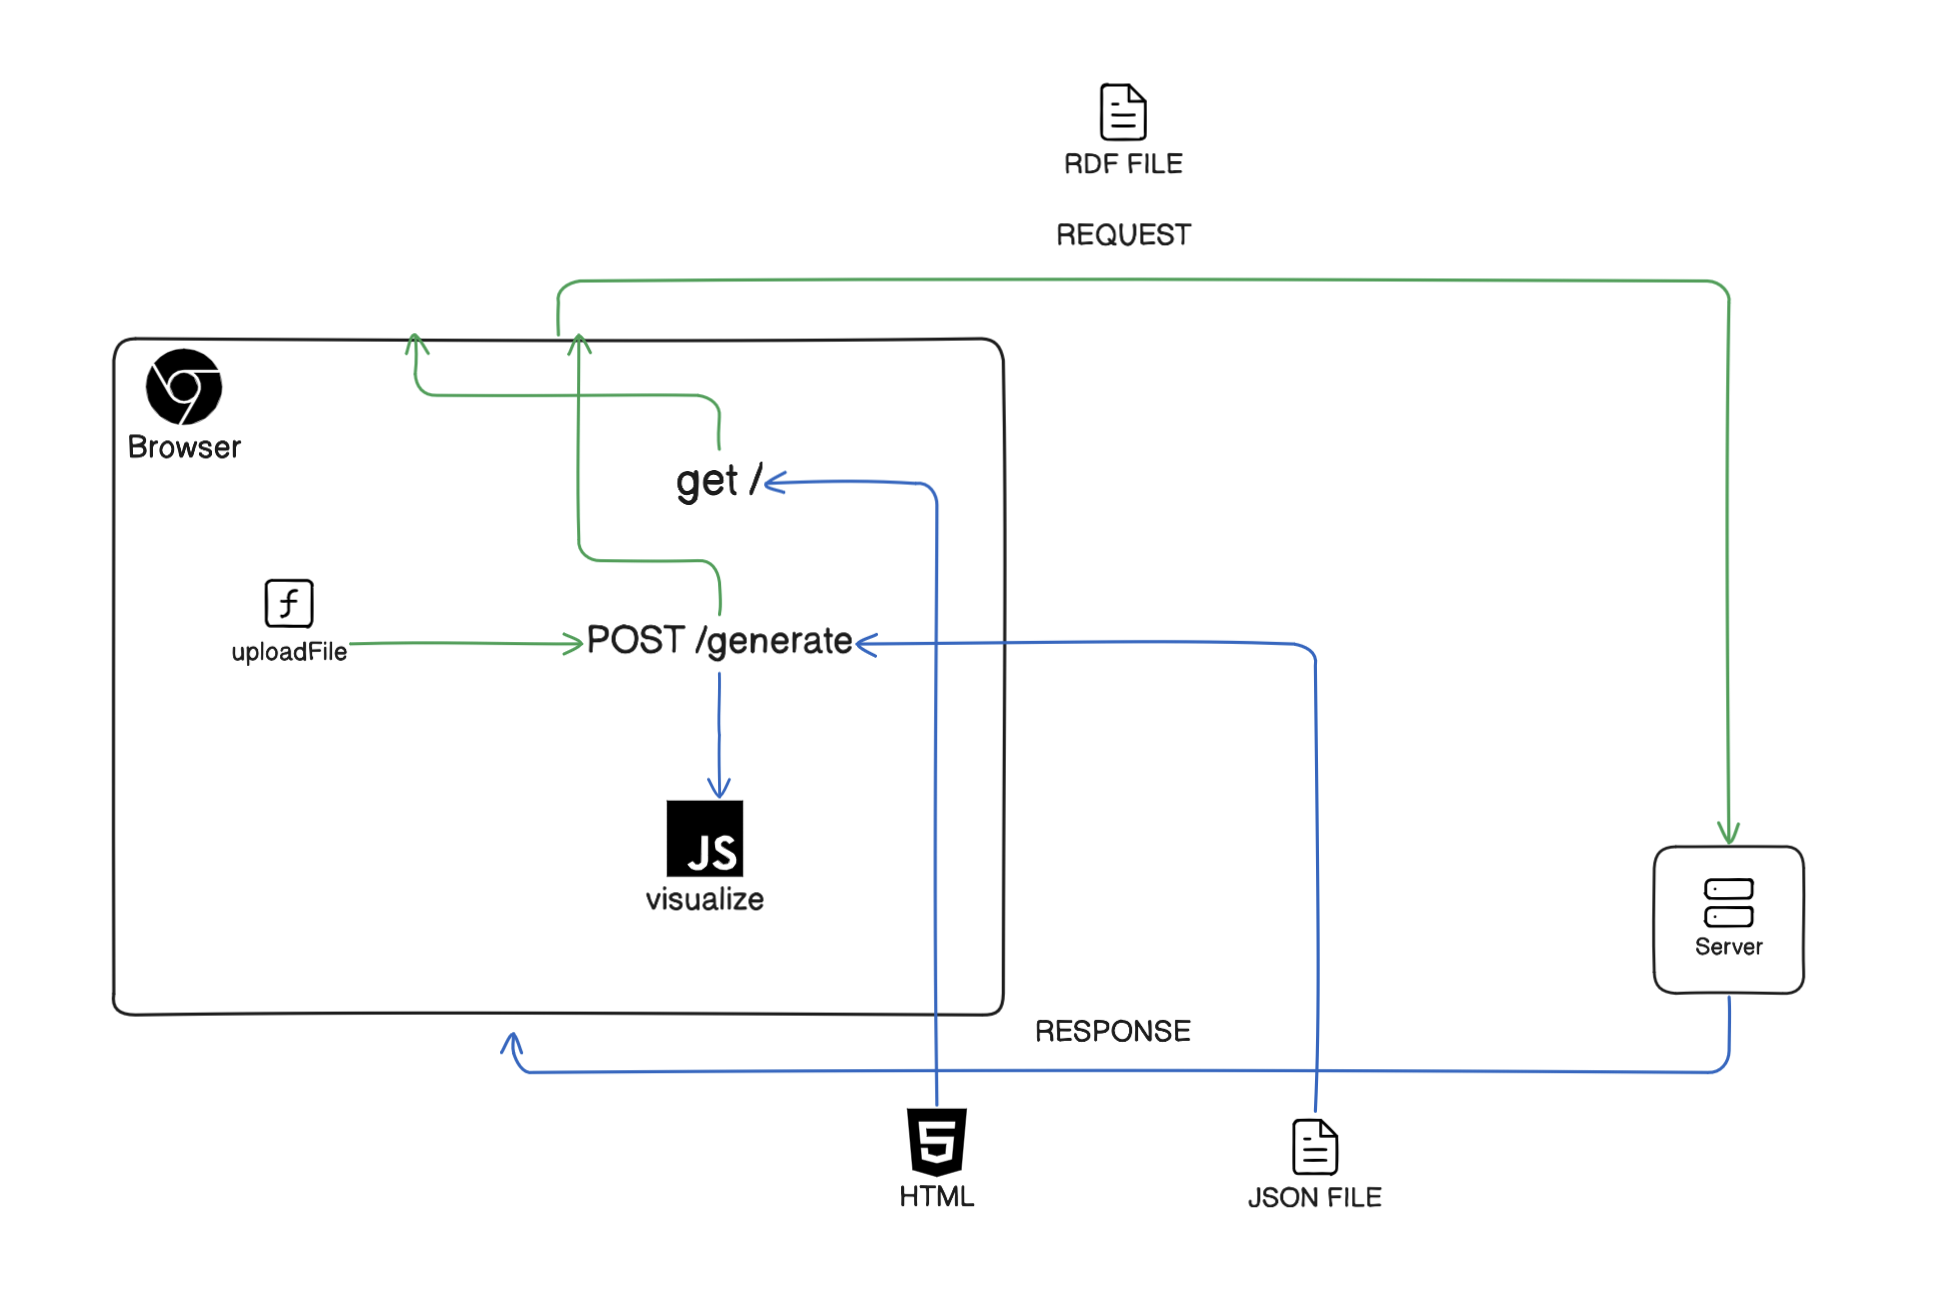
\includegraphics[width=13cm]{dataflow-browser-rdf-request.png}
	\caption{Web extension}
	\label{fig:dataflow-browser-rdf-request}
  \end{figure}
\subsection{The Fetch}
When the user wants to use the RDF Instance Generator and Visualizer, the fastest way is by doing via a web browser. 
\\
By simply getting the default route ($/$) of the server, an HTML page is retrieved. This page allows to upload a RDF file to the server ($/generate$ route). 
Upon a successful upload, the page allows to read the new generated RDF file and renders the json-dl graph, thanks to the support of the vis.js library. 
The following describes the pipeline for the conversion from json-dl into an interactive RDF graph.

\subsection{Graph Rendering}
When the $index.html$ file renders, it loads two main javascript files: the $uploader.js$ and the $visualizer.js$.
The first one, generate a web component (the $TurtleFileUploader$), that allows to upload a file and make POST requests. Upon receiving a positive response, the component injects the json-dl data into the custom rdf-visualizer as jsondata attribute. 
Furthermore, the response data ($res.data$), containing the new RDF file with the new generated instance is then attached to the DOM, so the user can inspect and download the upgraded version of its RDF.
\\
\\
\begin{lstlisting}[caption={\texttt{TurtleFileUploader} component}, label={lst:turtle-file-uploader}, language=JavaScript]
	class TurtleFileUploader extends HTMLElement {
	  constructor() { ... }
	
	  connectedCallback() { ... }
	
	  async uploadFile(edit = false, search = false) {
		const fileInput = this.shadowRoot.getElementById("fileInput");
		const responseDiv = this.shadowRoot.getElementById("response");
		const rdfVisualizer = document.getElementById("rdfVisualizer");
		const n = this.shadowRoot.getElementById("n").value;
	
		if (fileInput.files.length === 0) { ... }
	
		if (search && n > 3) { ... }
	
		const formData = new FormData();
		formData.append("file", fileInput.files[0]);
	
		try {
		  const response = await fetch(`/generate?n=${n}&edit=${edit}&property_search=${search}`, {
			method: "POST",
			body: formData
		  });
	
		  if (!response.ok) throw new Error(`HTTP error! Status: ${response.status}`);
	
		  const res = await response.json();
		  responseDiv.innerText = res.data;
	
		  const blob = new Blob([res.data]);
		  const url = URL.createObjectURL(blob);
		  const a = document.createElement("a");
		  a.href = url;
		  a.download = res.fileName;
		  a.innerText = `Download ${res.fileName}`;
		  a.style.display = "block";
		  responseDiv.appendChild(a);
	
		  rdfVisualizer.setAttribute("jsondata", res.json_dl);
		} catch (error) {
		  responseDiv.innerHTML = "Error: " + error.message;
		}
	  }
	}
	
	customElements.define('turtle-file-uploader', TurtleFileUploader);
	\end{lstlisting}
	

The second, the rdf-visualizer component, listen to this attribute and triggers a parsing function to safely deserialize the data. To ensure coherence and render compatibility, the data is normalized into an array of RDF subject objects, each containing an id, type, and property-value pairs.
\\
\\
The core conversion from RDF semantic to a network compatible logic is done by the $processJsonLd$ function. 
Every RDF subject is converted into a node and the classified as a Class (rdfs:Class rendered as orange boxes), a Property (rdf:Property represented as green-yellow diamonds), an Instance (URI-based entities shown as blue dots) or a Literal (visualized as yellow box).
\\
\\
\begin{lstlisting}[caption={\texttt{processJsonLd} function used for graph construction}, label={lst:rdf-visualizer}, language=JavaScript]
	function processJsonLd(data, dynamicPrefixes) {
	  const nodesMap = {};
	  const edges = [];
	  let literalCounter = 0;
	
	  data.forEach(item => {
		const subjectId = item['@id'];
		let nodeType = 'instance';
	
		// Type classification
		if (item['@type']) {
		  const types = Array.isArray(item['@type']) ? item['@type'] : [item['@type']];
		  if (types.includes("...#Class")) nodeType = 'class';
		  else if (types.includes("...#Property")) nodeType = 'property';
		}
	
		// Subject node creation
		if (!nodesMap[subjectId]) {
		  let label = item["...#label"] ? item["...#label"][0]["@value"] : shorten(subjectId, dynamicPrefixes);
		  let shape = nodeType === 'class' ? 'box' : nodeType === 'property' ? 'diamond' : 'dot';
		  let color = nodeType === 'class' ? '#FFA500' : nodeType === 'property' ? '#ADFF2F' : '#97C2FC';
		  nodesMap[subjectId] = { id: subjectId, label, shape, color, baseColor: color, nodeType, font: { color: "#000000" } };
		}
	
		// Type edge creation
		if (item['@type']) {
		  types.forEach(t => {
			let typeId = typeof t === 'string' ? t : t['@id'];
			if (typeId && !nodesMap[typeId]) {
			  nodesMap[typeId] = { id: typeId, label: shorten(typeId, dynamicPrefixes), shape: 'box', color: '#FFA500', ... };
			}
			edges.push({ from: subjectId, to: typeId, label: shorten("...#type", dynamicPrefixes), dashes: true, color: { color: '#000' } });
		  });
		}
	
		// Property edges and literal nodes
		Object.keys(item).forEach(prop => {
		  if (prop === '@id' || prop === '@type') return;
		  item[prop].forEach(val => {
			if (val['@id']) {
			  if (!nodesMap[val['@id']]) nodesMap[val['@id']] = { id: val['@id'], label: shorten(val['@id'], dynamicPrefixes), shape: 'dot', ... };
			  edges.push({ from: subjectId, to: val['@id'], label: shorten(prop, dynamicPrefixes), arrows: 'to', ... });
			} else if (val['@value']) {
			  const literalId = `literal_${literalCounter++}`;
			  nodesMap[literalId] = { id: literalId, label: String(val['@value']), shape: 'box', color: '#FFD700', ... };
			  edges.push({ from: subjectId, to: literalId, label: shorten(prop, dynamicPrefixes), arrows: 'to', ... });
			}
		  });
		});
	  });
	
	  return { nodes: Object.values(nodesMap), edges };
	}
	\end{lstlisting}
	
Each RDF triple is mapped to an edge between subject and object, labeled by the predicate. Type relationships (rdf:type) are highlighted with dashed edges to differentiate them from standard property connections.
\\
\\
After the nodes and edges definition, they are initialized into a vis-network object, the vis algorithm partially distribute the nodes onto the canvas. The graph is then stabilized to enhance readability and explorability. To improve furthermore the user experience, when a user clicks on a node, all the non-neighboring nodes are blurred out. 


\section{Implementation of the Visual Studio Code Extension}	


Visual Studio Code, initially intended as lightweight source code editor, has now evolved into a fully functional IDE thanks to its extensive ecosystem of plugins.
\\
Since VSCode it's built on top of Electron, a framework for building desktop applications using web technologies, it's possible to build extensions with the traditional web tolls (HTML, CSS, JavaScript).
\\
The following extension is built upon the Visual Studio Code Extension API, which provides a set of interfaces and classes to implement when working with the core capabilities of the editor.
\\
The following section describes the implementation of the Visual Studio Code extension with all its key features. 

\begin{figure}[htb]
	\centering
	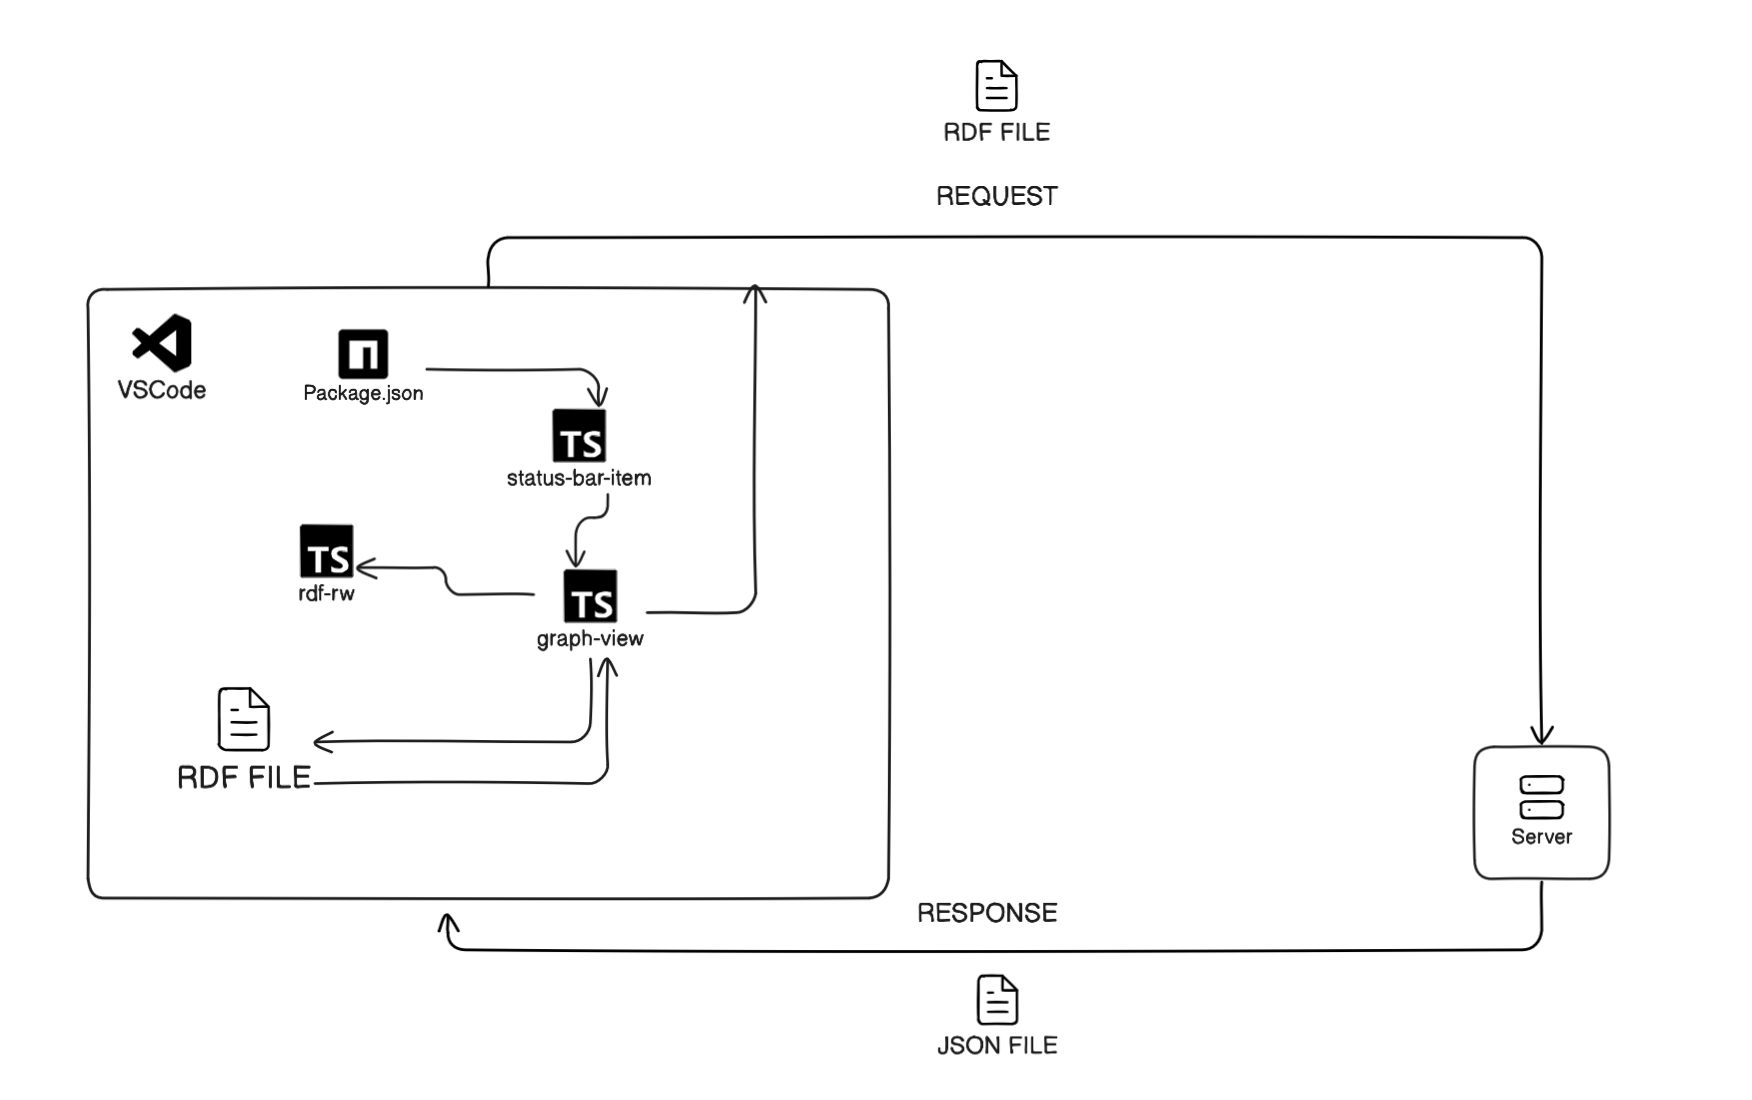
\includegraphics[width=13cm]{dataflow-vscode-extension.png}
	\caption{VSCode extension}
	\label{fig:vscode-extension}
  \end{figure}

\subsection{Commands Architecture}
Commands trigger actions in Visual Studio Code. In this case, commands have been used by the RIGVS extension to expose the following functionality to users: graph view ($extension.viewGraph$), simple instances generation and graph view ($extension.runGraph$) and instances generation with search properties and graph view ($extension.searchProperty$)

\begin{lstlisting}[caption={package.json commands declaration}, label={lst:commands-declaration}, language=JavaScript]
	...
	"commands": [
		{
		  "command": "extension.runGraph",
		  "title": "RIGSV generate instance & view graph"
		},
		{
		  "command": "extension.searchProperty",
		  "title": "RIGSV generate instance with properties"
		},
		{
		  "command": "extension.openMenu",
		  "title": "RIGSV Options"
		},
		{
		  "command": "extension.settings",
		  "title": "RIGSV settings"
		},
		{
		  "command": "extension.viewGraph",
		  "title": "RIGSV view graph"
		},
		{
		  "command": "extension.editRDF",
		  "title": "RIGSV edit RDF"
		}
	  ],
	  ...
	\end{lstlisting}

	Every command in VSCode can be executed by simply pressing $cmd + shift + p$. After the input dialog window opens up, each command present in the $package.json$ \ref{lst:commands-declaration} can be executed by typing the title and pressing the enter key. 
	\\
	\\
	The first command ($extension.viewGraph$) allows to open Webview inside the VSCode workspace. This webview renders the information coming from the server. 
	\\
	At the current project state, this command can be only executed while focusing the RDF file that needs to visualized as a graph. 
	When the command is executed, a new panel ($vscode.window.createWebviewPanel$) is generated with specific options (side panel view and enabling scripts execution inside the panel).
	After this the $getWebviewContent$ is called. 
	\\
	\\
	The \textbf{getWebviewContent} function prepares the web view for the graph visualization. It executes the $sendRDFContent$ function, that allows to extract data from the file focussed by the user ($getRDFContent$) and to send it to the server. 
	After getting the response, static urls for the incoming scripts ($visualizer.js$ and $uploader.js$) and then replaced in the html file.
	\\
	Since VSCode Webviews are intended to load HTML content in a sandboxed environment, the default CSP (Content Security Policy) is restricting external resources like scripts and external stylesheets. 
	\\
	Including the following meta tag in the head of the html content returned by $getWebviewContent$ is essential to implement a runtime Content Security Policy that permits script execution. The necessary adjustments are stored in the $csp$ variable:
	\\
	\\
	\texttt{<meta http-equiv="Content-Security-Policy" content="\$\{csp\}">}
	\\
	\\
	After the content is returned, it is rendered in the webview panel. The page also listed for 2 specifics clicks events: the \textbf{editButton} and the \textbf{exportGraph}.
	When the user clicks on the edit button, the $extension.editRDF$ commands is triggered. This opens the new RDF graph in the VSCode editor, in the original RDF format. 
	\\
	The $extension.exportGraph$ command is used to export the graph in a png format.
	\\
	\\
	The second command ($extension.runGraph$) has the exact same features as the previous command.
	After its execution and additional input element appears as pop window and requires the amount of instances that need to be generated by the server.
	\\
	The last one ($extension.searchProperty$) has the exact same behavior of the previous one, but with addiction of the properties search functionality.
	\\
	\begin{lstlisting}[caption={openWebView}, label={lst:open-web-view}, language=JavaScript]
		export function openWebView(context: vscode.ExtensionContext) {
			const viewGraph = vscode.commands.registerCommand(
			  "extension.viewGraph",
			  async () => {
				vscode.window.showInformationMessage("Graph view is loaded");
		  
				let panel = vscode.window.createWebviewPanel(
				  "rdfVisualizer",
				  "RDF Visualizer",
				  vscode.ViewColumn.Beside,
				  {
					enableScripts: true,
					retainContextWhenHidden: false,
				  }
				);
		  
				if (envConfig.serviceEndpoint) {
				  const htmlContent = await getWebviewContent(
					panel.webview,
					envConfig.serviceEndpoint,
					true
				  );
				  panel.webview.html = htmlContent;
				}
		  
				panel.webview.onDidReceiveMessage(
				  async (message) => {
					if (message.command === "editRDF") {
					  vscode.commands.executeCommand("extension.editRDF");
					}
				  },
				  undefined,
				  context.subscriptions
				);
				exportGraph(panel)
			  }
			);
		 const runGraph = vscode.commands.registerCommand(...)
			const searchProperty = vscode.commands.registerCommand(...)
			const editRDFCommand = vscode.commands.registerCommand(...)
			...
		}
		\end{lstlisting}
	At the current project state, this command can be only executed while focusing the RDF file that needs to be enhanced
	\\
	To facility the access to these commands, a quick menu button has been design. The button locates at the button right corner of the VSCode window. By click the button a modal with a simple select allows the selection between these three commands. 

\section{Implementation of the IntelliJ IDEA plugin}	

The following section describes the implementation of the IntelliJ IDEA plugin with the showcase of the feature. 

\begin{figure}[htb]
	\centering
	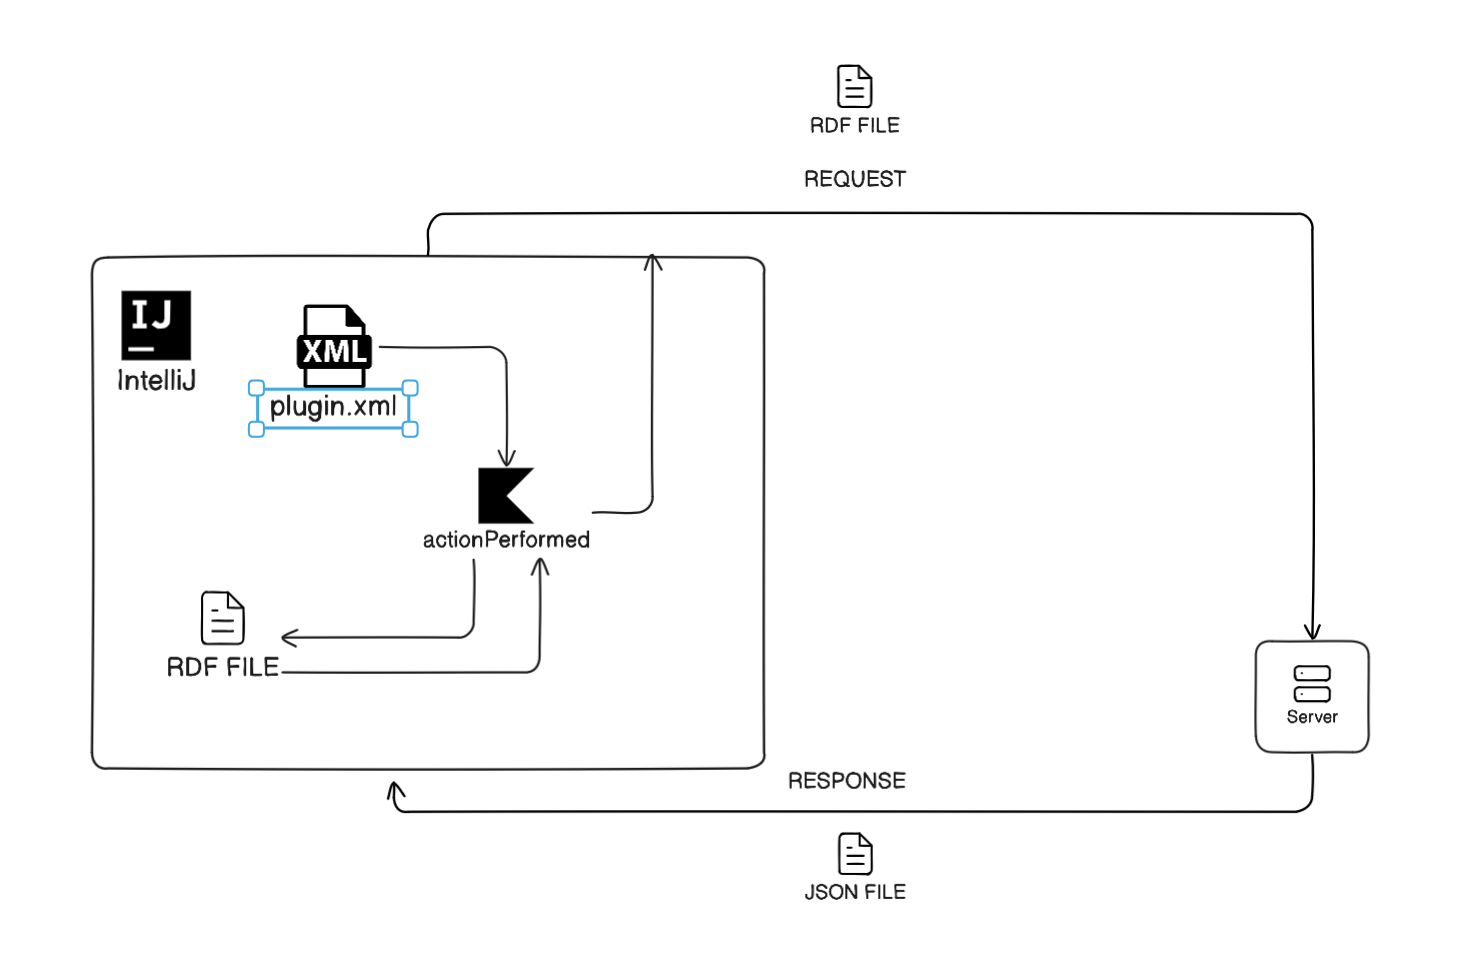
\includegraphics[width=13cm]{dataflow-intellij-extension.png}
	\caption{IntelliJ Extension}
	\label{fig:intellijextension}
  \end{figure}

Like the VSCode extension, the goal of the IntelliJ IDEA plugin is to provide a user-friendly interface for generating RDF instances and visualizing them in a side panel as graph.
This extension, developed mainly for the pourpuse of demonstrating the flexibility of this tool's architecture as a distributed system, only has implemented the feature responsible for rendering the RDF Graph in a side panel.
\\
\\
The extension is developed using Kotlin programming language, Glade plugin manager and the JetBrains Plugin DevKit.
\\
Like the VSCode world, the IntelliJ IDEA plugin has \textbf{actions} ($commands$ in VSCode) that allow to execute functions, based on users input.
\\
\\
\begin{lstlisting}[caption={IntelliJ Actions}, label={lst:actions}, language=xml]
<?xml version="1.0" encoding="UTF-8"?>
<idea-plugin>
    <id>com.example.rdf</id>
    <name>RDF Visualizer</name>
    <vendor>Wesley G. Obi</vendor>
    <description>Visualizing RDF Files Graphically Using an External Python Service</description>

    <depends>com.intellij.modules.platform</depends>

    <actions>
        <action id="RDFVisualizer.Convert"
                class="com.example.rdf.RDFVisualizerAction"
                text="Visualize RDF"
                description="Converts the current RDF file into a graphical visualization">
            <add-to-group group-id="EditorPopupMenu" anchor="last"/>
        </action>
    </actions>
</idea-plugin>
\end{lstlisting}

When a user right-clicks on an RDF file, the \textbf{Visualize RDF} action now appears in the right-click menu.
\\
\\
\begin{figure}[htb]
	\centering
	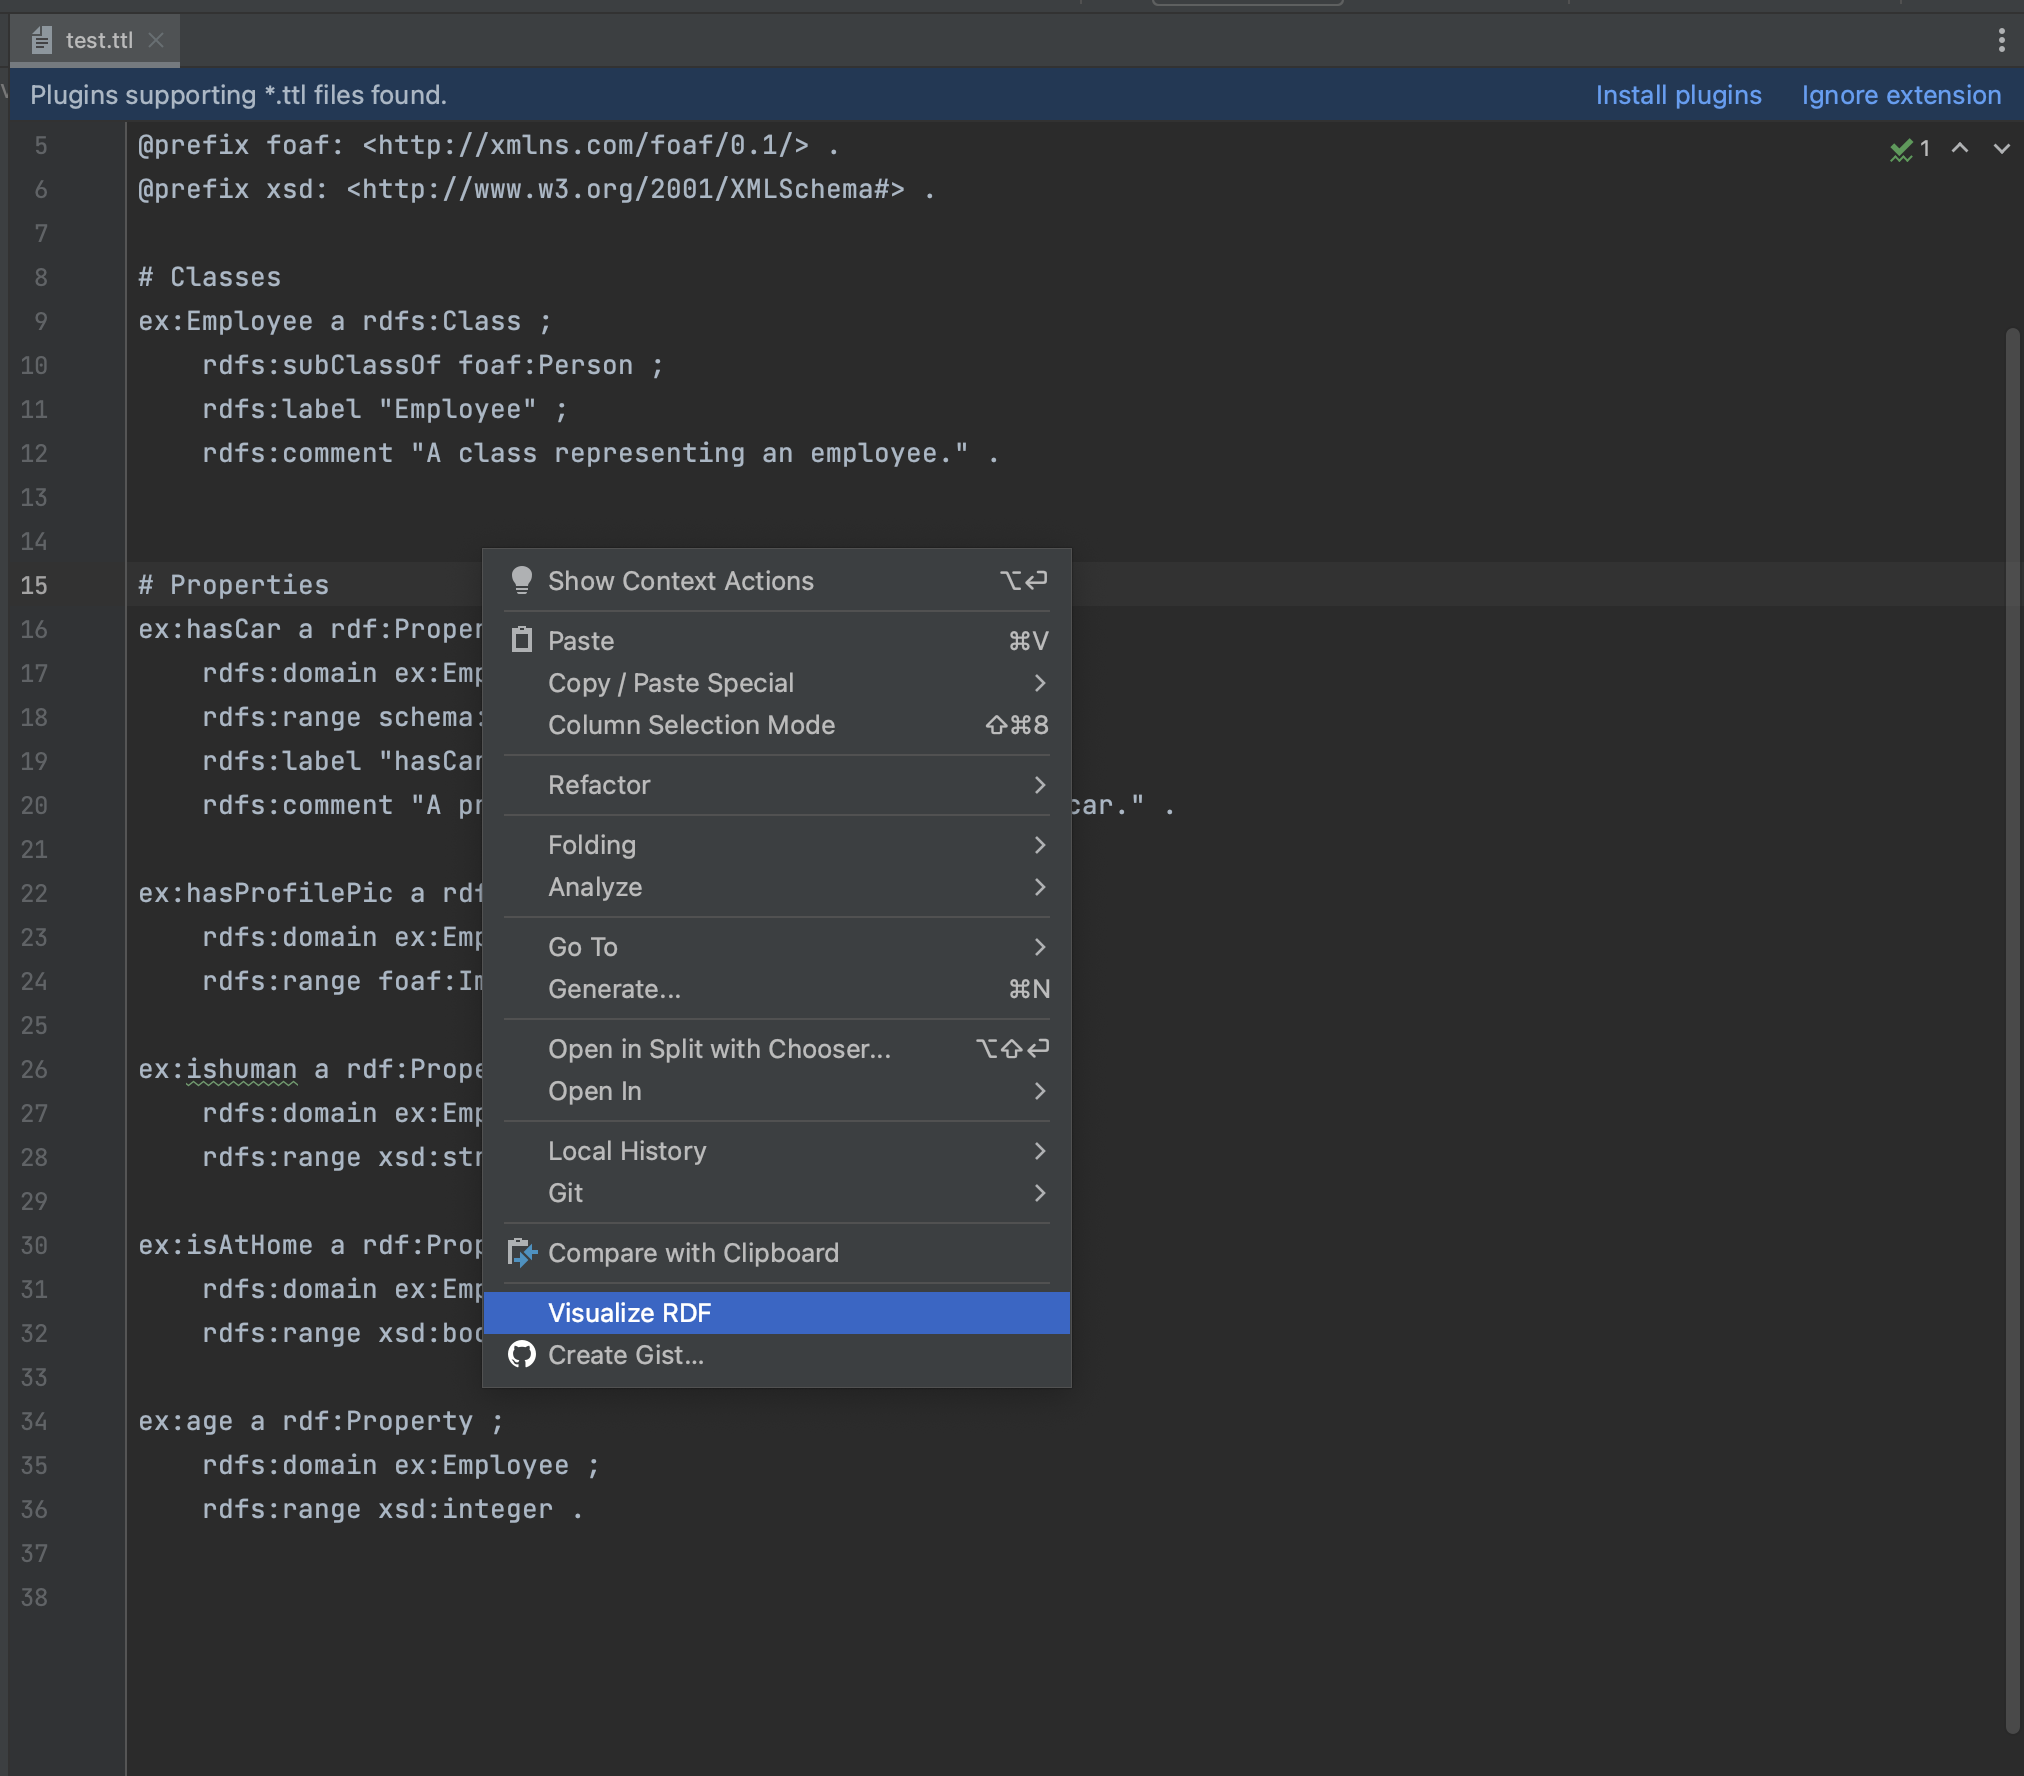
\includegraphics[width=14cm]{actioncallinintellij.png}
	\caption{Action call in IntelliJ}
	\label{fig:actioncallinintellija}
  \end{figure}

By simply clicking on it the action gets triggered and executes the $actionPerformed$ function. 
\\
This function extracts the RDF scheme from the focused file, and wraps in a formData object. Then, it sends the relevant information to the python server. 
The response is then passed to the $showGraphViewer$ function, responsible for rendering the graph in a side panel.
Just like in the VSCode extension, the html contet is processed to ensure that CSP restrictions are removed and resources can be called and rendered inside the Intellij Web view. 
\\
\\
\begin{lstlisting}[caption={Render graph in WebView in IntelliJ}, label={lst:open-web-view-intellij}, language=Java]
override fun actionPerformed(e: AnActionEvent) {
	...
	val formData = MultipartBody.Builder()
		.setType(MultipartBody.FORM)
		.addFormDataPart("fileUpload", file.name, requestBody)
		.build()

	val request = Request.Builder()
		.url("http://localhost:8000/")
		.post(formData)
		.build()

	val client = OkHttpClient()

	try {
		val response = client.newCall(request).execute()
		if (response.isSuccessful) {
			val jsonResponse = response.body?.string() ?: throw Exception("Empty response body")
			val responseBody: ServerResponse = Json.decodeFromString(jsonResponse)

			showGraphViewer(project, responseBody.content)
		} else {...}
		...
	}
}
\end{lstlisting}

\section{Documentation and Deployment Architecture\label{sec:docu}}
The documentation of the project is available in the GitHub repository in the $README.md$ file. 
In there are listed two type if installation: the Developer installation and the User installation. 
\\
\\
For the first one, developers need to install all the relevant programming languages, runtimes and dependencies (Python, Node.js, pip, npm, etc.). 
They need also to start the python server and the extension inside the VSCode development environment.
\\ 
\\
For the end user it actually much simpler. The repository already includes a build version of the VSCode extension that can be installed like any other extension. 
\\
To make the web service compatible with every machine in the world, it has been dockerized so that also the end user doesn't need to manually download additional tools other than Docker desktop.


